\documentclass[a4paper]{ltxdoc}
% \usepackage[margin=2cm]{geometry}
%% Fonts, etc.

%% Language and font encodings
\usepackage[english]{babel}
%\usepackage[utf8x]{inputenc}
%\usepackage[T1]{fontenc}        
% \usepackage{microtype}      % fine pdf font control

% \usepackage[scaled=0.92]{helvet} \renewcommand{\familydefault}{\sfdefault}
% \usepackage{xcolor} -- loaded by tikz
% \usepackage{soul} % \ul \st \hl

%% packages from beamer user guide
\usepackage{cmap}
\usepackage{lmodern}
\usepackage[T1]{fontenc}
\usepackage[utf8]{inputenc}
\usepackage{amsmath,amssymb}
\usepackage{pifont}
\usepackage{makeidx}
\usepackage{pgf,xcolor}
\usepackage[pdfborder={0 0 0},bookmarksnumbered]{hyperref}
\usepackage[left=2.25cm,right=2.25cm,top=2.5cm,bottom=2.5cm,nohead]{geometry}
\usepackage{translator}
\usepackage{tikz}
\def\TikZ{Ti\textit{k}Z}

%% beamer userguide macros
\input{beamerug-macros}

% adapt the environment doc macro to provide environment contents
\makeatletter
\def\envwithcontents#1#2{\list{}{\leftmargin=2em\itemindent-\leftmargin\def\makelabel##1{\hss##1}}%
  \extractflexenvironement#1@{#2}\par\topsep=0pt}
\def\endenvwithcontents{\endlist}
\def\extractflexenvironement#1#2@#3{%
\item{{\ttfamily\char`\\begin\char`\{\declare{#1}\char`\}}#2}%
  {\itemsep=0pt\parskip=0pt%
    {\itemindent=-1em #3}%
    \item{\ttfamily\char`\\end\char`\{\declare{#1}\char`\}}%
  }%
  \index{#1@\protect\texttt{#1} environment}%
  \index{Environments!#1@\protect\texttt{#1}}}
\makeatother


%% Maths
\usepackage{amssymb,amsmath}
% \usepackage{algorithm,algpseudocode}
% \usepackage{mathtools}
% \usepackage{mathalfa}
% \usepackage{bbm}
% \usepackage{mathrsfs}
% \usepackage{gensymb}
% \input m.macros
% \input m.symbols

%% Other typsetting
% \usepackage{booktabs}       % professional-quality tables
% \usepackage{nicefrac}       % compact symbols for 1/2, etc.
% \usepackage{enumerate}

%% Graphics
% \usepackage{graphicx,tikz}
% \usetikzlibrary{positioning}
% \usetikzlibrary{fit}
% \usetikzlibrary{calc}

%% Floats
% \usepackage{wrapfig}

%% Margin bubbles
% \usepackage{mbubble}
% \mbubblestyle{ms}{font=\tiny,label=ms,color=blue}
% \newcommand{\comment}[1]{}

%% Sections
% \usepackage{titlesec} % format section titles
% \titleformat{command}[shape]{format}{label}{sep}{before-code}[after-code]

% \usepackage{caption,subcaption}
% \DeclareCaptionSubType[Alph]{figure}
% \captionsetup[subfigure]{labelformat=simple,labelfont={sf,bf,large},textfont={sf}}
% \renewcommand{\thesubfigure}{{\sffamily\alph{subfigure}}}

%% Spacing
% \usepackage[doublespacing]{setspace}
% \parindent 0pt
% \parskip 1ex

%% Citations, refs, hyperlinks
% \usepackage[colorlinks=true, allcolors=blue]{hyperref}
% \usepackage{natbib}
\usepackage[capitalize]{cleveref}
% \crefname{equation}{}{}
% \crefname{Equation}{Equation}{Equations}



%% Title

\title{Enhanced \beamer\ increments:\\
the \texttt{beamincr} package}
\author{Maneesh Sahani}
\date{\today}
% \usepackage{filemod} % access to file modification times
% \date{\Filemodtoday{\jobname}}  % replace \jobname if compiling from wrapper

% \usepackage{titling} % modify title(page) appearance
%\pretitle{\begin{center}\LARGE}
%\posttitle{\par\end{center}\vskip 0.5em}
%\preauthor{\begin{center} \large \lineskip 0.5em \begin{tabular}[t]{c}}
%\postauthor{\end{tabular}\par\end{center}}
%\predate{\begin{center}\large}
%\postdate{\par\end{center}}



%% Document


\begin{document}

\maketitle

\noindent
The |beamincr| package provides a set of extensions and enhancement to the
incremental overlay mechanisms implemented in the \beamer\ class.  These
include labels to refer to and manipulate overlay steps, an extended action
syntax, and new increment-aware environments.

\section{Background: overlays and increments}

The basic \beamer\ display unit is the \texttt{frame}.  A
frame may be rendered step-by-step, in which case the individual
versions of the frame are called ``overlays'' or ``slides''.  We will
use these terms interchangeably.
%
\beamer\ allows you to place material on an arbitrary slide in a frame like this
\example
\begin{verbatim}
\begin{frame}
  text on slides 1 and up\\
  \onslide<2->
  text on slides 2 and up\\
  \onslide<3-4>{
  text only on slides 3 and 4\\
  } 
  \only<5>{text only on slide 5\\}
  more text on slides 2 and up\\
\end{frame}
\end{verbatim}
You can read about the differences between \myprintcommand{onslide}
and \myprintcommand{only}, and the many other overlay-sensitive
commands, in the \beamer\ user guide.  Note in particular the
difference between the argument form and the declaration forms of
\myprintcommand{onslide}.  \myprintcommand{only} only works with an
argument.

This explicit numbering approach becomes burdensome when you want many overlays.
You have to keep track of the numbers explicitly, and if you subsequently add a
step early in the sequence you need to re-number the rest.  Thus, \beamer\ also
provides an incremental overlay specification.  The following code will produce
the same effect as that above.  \example
\begin{verbatim}
\begin{frame}
  \resetincr % not standard BEAMER
  text on slides 1+\\
  \onslide<+->
  text on slides 2+\\
  \onslide<+-+(1)>{ % increments counter by 1, despite the two +s
  text only on slides 3-4\\
  } 
  \onslide<+>{} % increment counter by another
  \only<+>{text only on slide 5\\}
  more text on slides 2+\\
\end{frame}
\end{verbatim}
This form allows easy automation using default overlay specifications.  For
instance (from the \beamer\ user guide) \example
\begin{verbatim}
\begin{itemize}[<+-| alert@+>]
\item Apple
\item Peach
\item Plum
\item Orange
\end{itemize}
\end{verbatim}
There are important and sometimes not-entirely-intuitive differences between the
incremental and explicit numbering systems.  So we will refer to the steps
implied in this way as ``increments''.  They will mostly match slide numbers,
but not always, as this example shows: \example
\begin{verbatim}
\begin{frame}
  \resetincr % not standard BEAMER
  text on slide 1+\\
  \onslide<3>{text on slide 3}\\
  text on slide 1+\\
  \onslide<+->
  text on slide 2+\\
  \onslide<4->
  text on slide 4+\\ % increment number is still 2!
  \onslide<+->
  text on slide 3+\\
\end{frame}
\end{verbatim}
The increments have their own internal logic (specifically, their own internal
counter) which is not affected by any explicit slide specifications that may
appear in-between incremental calls.  It may make sense to think of the
increment number as being associated with \emph{where} in the source file the
material appears, rather than (necessarily) on \emph{which slide} it appears.

There are a couple of oddities with the way increments work that often trip up
first-time users.  There are also some extensions that would be nice, like the
ability to refer to a specific increment elsewhere in the frame.  These things
are certainly possible in stock \beamer, but take some digging into internals.
The tools here make things a bit easier.

As an aside, \beamer\ has another incremental overlay system based on the
|\pause| command.  This uses the same counter as increments (in fact, the
counter is called |beamerpauses|), but inteprets it slightly differently. This
difference is discussed in \cref{sec:internals}. As a result, the two sets of
specifications don't play very well together, at least from the viewpoint of
non-experts.  More on this below.  I strongly suggest avoiding
|\pause| entirely when using |beamincr|.


\section{Setting increments}\label{sec:setting}

\begin{command}{\resetincr\oarg{incr}}
  This command resets the increment number to 1, or to the value defined by
  \meta{incr} if given.  It doesn't directly affect the slide on which
  subsequent text appears, but it does change effect of subsequent |<+>| or
  |<.>| increments.  The command may be useful to synchronise overlays in (say)
  two columns or between highlighted bullet points and highlighting in a figure.
  \example
\begin{verbatim}
\begin{frame}
  \resetincr
  \begin{center}
    Two lists \onslide<+->{in sync}
  \end{center}
  \begin{columns}
    \begin{column}{.2\textwidth}
      \begin{itemize}[<+-| alert@+>]
      \item Apple \item Peach \item Plum \item Orange
      \end{itemize}
    \end{column}
    \begin{column}{.2\textwidth}
      \resetincr[2] % restart the increment counter to sync
      \begin{itemize}[<+-| alert@+>]
      \item green \item yellow \item purple \item orange
      \end{itemize}
    \end{column}
  \end{columns}
\end{frame}
\end{verbatim}
The argument \meta{incr} must either be a number or be an increment
specification enclosed in |/ /| (these are defined in \cref{sec:labels}).  It cannot specify any
sort of range, or be |+| or |.|, although |/./| and things like |/.(2)/| are
allowed.

It is useful to call |\resetincr| at the start of every increment-based slide
(as we have in the examples here).  This avoids some potentially confusing
behaviour that comes from the way the increment counter is implemented in
\beamer:
\example
\begin{verbatim}
\begin{frame}
  text on slides 1-\\
  \onslide<+->
  text still on slides 1-\\
  \onslide<+->
  text on slides 2-
  \resetincr\onslide<.->
  text on slides 1-\\
  \onslide<+->
  text on slides 2-
\end{frame}
\end{verbatim}
The first call to |\onslide<+->| doesn't advance the slide, unless it has been
preceded by a |\resetincr| (or another |\onslide<+->| or a |\pause|).
\end{command}

\begin{command}{\fromincr\sarg{incr}}
  This is shorthand for
\begin{verbatim}
\resetincr[incr]
\onslide<.->
\end{verbatim}
It can only be used as a declaration (not with an argument).  The restrictions
on \meta{incr} are the same as above.  
\end{command}


\section{Labelling and referring to increments}\label{sec:labels}

In complicated frames, it may be useful to name certain increments for reference
elsewhere.  For instance, one might want to change a figure at certain steps
while progressing through a list of bullet points.  Or one might want to
redisplay certain slides in the frame with |\afterframe| or |\handoutframe|
(described below).

\begin{command}{\incrlabel\sarg{incr}\marg{label}}
\end{command}
\begin{command}{\incrlabel\sarg{incr}\opt{\meta{=}}\texttt{/}\meta{label}\texttt{/}}
  By default, this command attaches the current increment number to the label
  \meta{label}.  Once defined, the labelled increment can be recovered in
  (almost) any overlay spec using the constructs discussed below.  The
  \meta{label} can contain most characters, but should not start with any of the
  characters |.!=| or contain any of |()-~|.

  The |=| in the second form is optional, but if it is present then the
  |/|\meta{label}|/| may be separated from the |=| by additional material, which
  will be left in place.  The label must appear at the same grouping
  level as the |\incrlabel=| command and before the end of the current paragraph.
  This is similar to the behaviour of the |=| action described in
  \cref{sec:actions:=}.

  If the optional \meta{incr} is provided, \meta{label} is set to its value.
  The restrictions on \meta{incr} are the same as for |\resetincr|: it can be a
  number or an increment specification.  This allows forms like
  |\incrlabel</.(2)/>{x}| to set |x| to the current increment + 2.  See the
  discussion of increment specifications below.

  If \marg{label} starts with a number in parentheses (e.g. |(2)x|) then this
  number is added to the current increment, or to the value of \meta{incr},
  to obtain the label value.  Thus, the effect of the command above can also be
  achieved by |\incrlabel{(2)x}|.  
\end{command}

\begin{command}{\incrref \marg{incr spec}}
  This command returns the increment number defined by increment specification
  \meta{incr spec} as described below.
\end{command}

\noindent
The general form of an increment specification is
\begin{command}{{increment specification}: |label|\opt{|(offset)|}}
  The label can be a string assigned by a call to |\incrlabel|, or the special
  label `|.|' which refers to the current increment (this is subtly different to
  the incremental overlay specification `|.|').  A further special label `|!|'
  is introduced in \cref{sec:actions:!}.  The \meta{offset}, if given, is
  added to the increment indicated by the label.  It can be negative.

  Increment specifications can be used as part of almost any overlay
  specification by enclosing them with slashes, e.g. |</mylabel(2)/>|.
\end{command}

An example:
\example
\begin{verbatim}
\begin{frame}[label=twolists]
  \resetincr
  \begin{center}
    Two lists \onslide<+->{in sync}\\
    \onslide<+->{with more material\\}
    \onslide<+->{at the top}
  \end{center}
  \begin{columns}
    \begin{column}{.2\textwidth}
      \incrlabel{startlist}%
      \begin{itemize}[<+-| alert@+>]
      \item Apple \item Peach \incrlabel{halfway} \item Plum \item Orange
      \end{itemize}
    \end{column}
    \begin{column}{.2\textwidth}
      \resetincr[/startlist/]% keep in sync, even if we add extra topmatter
      \begin{itemize}[<+-| alert@+>]
      \item green \item yellow \item purple \item orange
      \end{itemize}
    \end{column}
  \end{columns}
  \vfill
  \onslide<+->
  The final increment is \incrref{.}. 
  \incrlabel{end}
\end{frame}
\end{verbatim}

Note that of commands discussed here, |\incrref| expects an increment
specification (i.e. |label(offset)|), while |\resetincr|, |\fromincr| and
|\incrlabel| expect a restricted overlay specification that might be an
increment specification in |//| (e.g. |/label(offset)/|) or just a number.
Standard overlay-aware commands should all accept overlay specifications that
include increment specs.

One \beamer\ command (slightly patched in this package) with which named
increments are particularly useful is |\againframe|.  So \example
\begin{verbatim}
  \againframe<1,/halfway/,/end(-1)/-/end/>{twolists}
\end{verbatim}
provides an abbreviated tour of the lists.  Increment labels are associated with
the label of the enclosing frame, and so the same names can safely be reused
across multiple named frames.

There is also a similar new command called |\handoutframe| to render more than
one overlay from a frame in \texttt{handout} or similar modes that, by default,
just show a single slide with all the overlays collapsed.  See \cref{sec:helper}.

\section{Enhanced overlay action specifications}\label{sec:actions}

This section discusses further extensions to the overlay specification syntax,
and its interaction with increments and increment labels.


\subsection{Setting increments in overlay action specifications} \label{sec:actions:!}

It is possible to use the \beamer\ syntax for actions in overlays to reset the
increment number.  This can be done using the explicit |resetincr@|\meta{increment} action or
with an implicit |<!|\meta{increment}|>| specification.  \example
\begin{verbatim}
  \action<3-|resetincr@3>{body}
  \action<!3->{body}
\end{verbatim}
The increment number can be replaced by a label, with optional offset:
\begin{verbatim}
  \incrlabel<2>{x}
  \resetincr
  \action</x/->{body on 2+}
  \onslide<.->{this on 1+}
  \action<!/x(2)/->{body on 4+}
  \onslide<+->{this on 5+}
\end{verbatim}
The forms |<!+>| and |<!.>| aren't supported (and wouldn't be useful: |<+>|
already advances the increment, while |<!.>| would set it to its current value).
However |<!/.(|\meta{offset}|)/>| (note the |/| label notation) can be used to advance the
increment counter by multiple (or negative) steps.

The reset takes effect after the overlay specification has been interpreted and
before the body is set.  So any |+| or |.| references will be relative to the
increment in effect \emph{before} the |\action|.  However, the special increment
label |/!/| can be used to access the most recent reset.  \example
\begin{verbatim}
  \resetincr
  \action<!/.(2)/-|alert@.>{alert too early}
  \action<!/.(2)/->{\alert<.>{alert when uncovered}}
  \action<!/.(2)/-|alert@/!/>{alert when uncovered}
\end{verbatim}
It is possible to issue multiple |!| commands in one overlay spec but only the
first of them will take effect.

According to the user guide, \beamer\ actions are only supported by overlay
specifications to |\action|, |\item|, the |actionenv| environment and block
environments like |block| and |theorem|.  This package adds the fields of
incremental (\cref{sec:envs}) and incremental alignment environments
(\cref{sec:align}) to this list.  In the absence of any action specifications,
|\action| acts like |\uncover| (or |\onslide| with an argument).  Note that
|\fromslide| (\cref{sec:setting}) can act like an |\onslide| \emph{declaration} while
also setting the increment.

\subsection{Assigning labels from overlay action specifications} \label{sec:actions:=}

The \texttt{<$\cdots$\char`|=}\opt{\texttt{(}\meta{offset}\texttt{)}}\texttt{\char`|$\cdots$>} syntax can
be used to assign a label using an action specification.  The name of the label
to be assigned must be enclosed in \texttt{//}s within the \emph{argument} of
the |\action| (or |\item| or |\next| or alignment field
\dots)\footnote{\beamer\ actions don't make it possible to pass a text argument
  to the handler.}  The label is assigned to the increment number after any
\texttt{+} or \texttt{!} actions have been interpreted, as though it was called
with |\incrlabel| in place.  Thus in this code \example
\begin{verbatim}
  \resetincr[3]
  \action<!/.(2)/>{\incrlabel{x}action text}
  \resetincr[3]
  \action<!/.(2)/|=>{/x/action text}
  \resetincr[3]
  \action<!/.(3)/>{\incrlabel</.(-1)/>{x}action text}
  \resetincr[3]
  \action<!/.(3)/|=(-1)>{/x/action text}
  \resetincr[3]
  \action<!/.(3)/|=>{/(-1)x/action text}
\end{verbatim}
the first two action calls set the label \texttt{x} to 5.  The last three
illustrate the use of assignment offsets: if \texttt{=} is followed by a number
in parentheses, this is treated as an offset to add to the current increment at
assignment, in the same way as indicated by the optional |<|\meta{incr}|>|
argument to |\incrlabel|.  The same effect can be achieved by placing the offset
before the label name within the enclosing \texttt{//}.

If no \texttt{/label/} is found or if the name is empty, the action tries to do
nothing quietly.  This makes it possible to use an \texttt{=} in a default spec,
but only assign a label on selected steps.  However, this behaviour comes with
warnings, and should be used with caution.  First, because of the way \beamer's
internals work, it is not currently possible to omit the \texttt{//} in an
|\item|, although the label can be empty (omission is fine in the fields of an
incremental or incremental alignment environment).  Second, if there happens to
be one more or more \texttt{/} characters in the argument to the action, the
text between them (or from a single \texttt{/} to the end) will be interpreted
as a label, unless an explicit \texttt{//} pair appears first.  You have been
warned!

\subsection{Extending default overlay or action specifications} \label{sec:actions:~}

By default, explicit overlay or action specifications override any defaults that
might apply.  It may sometimes be convenient to instead extend the default.  The
|~| spec can be used to add the current default spec fields into an explicit
overlay specification.
\example
\begin{verbatim}
  \begin{itemize}[<+-| alert@+|=>]
  \item/ap/ Apple \item/pe/ Peach \item/pl/ Plum \item/or/ Orange
  \end{itemize}
  \begin{itemize}[<alert@/!/>]
  \item<!/pe/-|~> yellow \item<!/or/-|~> orange \item<!/ap/-|~>green \item<!/pl/-|~> purple
  \end{itemize}
\end{verbatim}
Within incremental alignment environments (\cref{sec:align}), a |~| will
incorporate the field-specific default.


\subsection{Advanced references: using labels defined later} \label{sec:actions:advanced}

\begin{command}{\allowundefinedincrlabels\oarg{flag}}
  If called alone, or with option \meta{\opt{flag}} > 0, tells \LaTeX\ not to
  generate an error when encountering an undefined increment label.  References
  to such labels instead evaluate to 0, and any offset in the reference is
  ignored.  If \meta{\opt{flag}}=0, the default error-generating behaviour is
  restored.
\end{command}
If a referenced label is defined later in the same frame, then it will take on
that later-defined value on subsequent slides of the frame.  Thus, in effect,
this option makes it possible to refer to increment labels before they are
defined.  (Although material intended to be set on slide 1 cannot depend on such
advance references.)

If the label is used as part of an open range then it may be necessary to use a
special syntax in which the range indicator is placed \emph{within} the |//|
enclosing the label.  If the label is undefined (and so 0), this syntax sets the
other limit of the range to 0 as well.
\example
\begin{verbatim}
  % /foo/ is not defined on first evaluation
  \onslide</foo/->{spec expands to <0->, so text appears on all slides}
  \onslide</foo-/>{spec expands to <0-0>, so text is suppressed}
  \incrlabel<2>{foo} % on later evaluations, both specs will expand to <2->
\end{verbatim}
If the range is closed with an explicit numerical or (defined) label upper
limit, then there is no current way to suppress early expansion.  However forms
like |/foo/-/foo(2)/| will evaluate to |0-0| as offsets are ignored for
undefined labels.

Many problems with advanced references (including range expansion and the
rendering of first-slide material) can be resolved by use of |\framescanonly|
and |\againframe| (\cref{sec:helper}).

An |\allowundefinedincrlabels| command also makes it possible to \emph{set} the
current increment to an (initially) undefined label value using |\resetincr|,
|\fromincr| or |<!/label/>|, thereby setting the current increment to 0.  Text
set on that increment will not appear until the label is defined.  However, any
subsequent |<+>| specs will still advance the increment number, which may not be
desired.  This behaviour can be avoided by using the form |<!/.(1)/>| instead of
|<+>|.  The current increment label |/./| is treated in the same way as an
undefined one when the increment is 0, and so the offset is ignored.
\example
\begin{verbatim}
\resetincr{/foo/} % no list items appear until /foo/ is defined
\begin{itemize}<!/.(1)-/|alert@/!/>
\item foo
\item bar
...
\end{itemize}
\end{verbatim}
If an initially undefined label is used to set the increment counter early in
the frame, then increment labels that are defined later in the frame may change
value once that first label is defined.  This can be used for powerful effects,
in which overlays in two different sections of the frame each depend on
increments from the other.  However, if the definition label used in the early
reference is itself altered by the change in that early evaluation, then there
is a risk of creating an infinite loop.
\example
\begin{verbatim}
  \begin{itemize}[<alert@/!/>]
  \item<!/./-     |~|=(1)>/ping/ Apple  % 1- (!/./ ensures alert occurs on same slide)
  \item<!/pong-/  |~> Peach             % 4-
  \item<!/.(1)-/  |~|=>/ping2/ Plum     % 5-
  \item<!/pong2-/ |~> Orange            % 8-
  \end{itemize}
  
  \begin{itemize}[<alert@/!/>]
  \item<!/ping-/  |~> green             % 2-
  \item<!/.(1)-/  |~|=(1)>/pong/ yellow % 3-
  \item<!/ping2-/ |~> purple            % 6-
  \item<!/.(1)-/  |~|=(1)>/pong2/orange % 7-
  \end{itemize}
\end{verbatim}



\section{Incremental environments}\label{sec:envs}

The |beamincr| package provides a set of new increment-aware environments.
These are described in the present section.  It also makes it possible to use
increment specifications within alignment environments such as |tabular| or
\AmSTeX\ |align|; these are discussed in \cref{sec:align}.

Each new environment is accessible under two, otherwise equivalent, names.  A
common base name is either preceded by the word \texttt{incremental} or followed
by the symbols \texttt{<>}.  The environments in this section separate material
into overlays using the token |\next| or |\next*|.  Many will also apply an
implicit or explicitly defined command to that material when |\next| is used,
but omit the command for |\next*|.

\subsection{Standard incremental environments}\label{sec:envs:incremental}

\begin{envwithcontents}{{incremental}
    \opt{\texttt{[<}\meta{default specification}\texttt{>]}}}
  {\item \hskip1em \sarg{pre-next specification} \opt{\meta{pre-next contents}}
    \item \texttt{\string\next}\sarg{next specification}
    \item \hskip1em \meta{next contents}
    \item \texttt{\string\next}\sarg{next specification}
    \item \hskip1em \meta{next contents}
    \item \hskip2em $\vdots$
  }
  This environment can be thought of as an increment-aware |itemize| without the
  list formatting.  This makes it suitable for incremental control of a wider
  range of types of code, such as \TikZ\ drawing commands.
%
  The keyword |\next| within the environment acts like |\item| in terms of
  incremental processing: the \meta{next contents} are set within an |\action|
  command.  Each |\next| call can be followed by an optional \sarg{next
    specification}, which is applied to the \meta{next contents}.  If the
  specification is omitted, then the environment \opt{\meta{default
      specification}} is applied.  If no \meta{default specification} was given
  in the environment, then the default is inherited from the frame or container
  default.  This is ordinarily |<*>|.

  Unlike in |itemize| environments, code can also appear before the first
  |\next|.  If any does, it is treated just like \meta{next contents}: it is
  executed with the action specification given by \sarg{pre-next specification}
  if present, or else the default specification.  On the other hand, if nothing
  but whitespace appears between the opening of the environment---or the
  optional default overlay spec---and the first |\next|) then no action is
  applied.  In particular, this avoids side effects from, e.g., |<+>|
  specifications in the default.  (This does not apply to later empty \meta{next
    contents}.)

  A counter called |next|, is set to 0 in the pre-next field and then advanced
  at every |\next|.
\example
\begin{verbatim}
\resetincr
\begin{incremental}[<+->]
  <.-> this text on slide 1;
\next
  on slide 2;
\next<!/.(2)/->
  on slide 4, but after only \theincrementalnext\ next commands.
\end{incremental}
\end{verbatim}
\end{envwithcontents}
\begin{environment}{{<>}\opt{\texttt{[<}\meta{default specification}\texttt{>]}}}
  This is a synonym for |\begin{incremental} ... \end{incremental}|.
\end{environment}
%
The following environments apply a specified command each overlay's contents.

\begin{envwithcontents}{{incrementaldo}
    \marg{command definition}\opt{\texttt{[<}\meta{default specification}\texttt{>]}}}
  {\item \hskip1em \sarg{pre-next specification} \opt{\meta{pre-next contents}}
    \item \texttt{\string\next}\sarg{next specification}
    \item \hskip1em \meta{next contents}
    \item \texttt{\string\next}\sarg{next specification}
    \item \hskip1em \meta{next contents}
    \item \hskip2em $\vdots$
  }

  This version treats each \meta{next contents} as the argument to a command.
  The command takes a single argument and is defined by \meta{command
    definition} in the same way as in |\newcommand|.  As the command evaluation
  happens deep within the bowels of \beamer\ processing, the single argument
  generally needs to be accessed as |####1|, \emph{unless} the enclosing frame
  is declared to be |fragile| (in the frame options), in which case it is just
  |#1|.

  The do command can be avoided for specific fields by using |\next*| in place
  of |\next|.  Contents following |\next*| are set in the same way as in a plain
  |incremental| environment.

  Any non-empty \meta{pre-next contents} is always processed without the do
  command.
  
\end{envwithcontents}
\begin{environment}{{do<>}\marg{command definition}\opt{\texttt{[<}\meta{default specification}\texttt{>]}}}
  This is a synonym for |\begin{incrementaldo} ... \end{incrementaldo}|.
\end{environment}


\begin{envwithcontents}{{incrementaldocmd}
    \oarg{num args}\marg{code}\opt{\texttt{[<}\meta{default specification}\texttt{>]}}}
  {\item \hskip1em \sarg{pre-next specification} \opt{\meta{pre-next contents}}
    \item \texttt{\string\next}\sarg{next specification}
    \item \hskip1em \meta{next contents}
    \item \texttt{\string\next}\sarg{next specification}
    \item \hskip1em \meta{next contents}
    \item \hskip2em $\vdots$
  }

   This version inserts \meta{code} (comprising arbitrary \LaTeX\ commands)
   after each |\next| and before \meta{next contents}.  If \meta{code} is (or
   ends with) a command that takes one or more arguments, these will be read
   from \meta{next contents}.  Braces may be needed within that text to
   delineate the arguments.

   If the optional \opt{\meta{num args}} is non-zero, then this number of
   arguments is read from the text following |\next| and can be accessed using
   argument parameters (almost) as in |\newcommand|.  As the command evaluation
   happens deep within the bowels of \beamer\ processing, the parameter numbers
   must be protected with four |####| symbols, \emph{unless} the frame is
   declared to be |fragile| (in the frame options) in which case a single |#|
   works.

  The \meta{code} can be avoided for specific fields by using |\next*| in place
  of |\next|.  Contents following |\next*| are set in the same way as in a plain
  |incremental| environment.

  Any non-empty \meta{pre-next contents} is always processed without \meta{code}.

  \example
\begin{verbatim}
\tikz[every node/.style={above,allow upside down,midway,sloped}]{
  \begin{incrementaldocmd}[1]{\draw ({72*\thenext-72}:10ex)--(72*\thenext:10ex) node {#1};}
                          [<+-|alert@+|=>]
    \next/one/   {one}
    \next/two/   {two}
    \next/three/ {three (\thenext/\theincrement)}
    \next/four/  {four}
    \next/five/  {five}
    \next*/done/ \draw (0:5ex) \foreach \t in {1,...,5}{ -- (\t*72:5ex)};
                 \node [anchor=center] {done!};
  \end{incrementaldocmd}}
\end{verbatim}
\end{envwithcontents}
\begin{environment}{{docmd<>}
    \oarg{num args}\marg{code}\opt{\texttt{[<}\meta{default specification}\texttt{>]}}}
  This is a synonym for |\begin{incrementaldocmd} ... \end{incrementaldocmd}|.
\end{environment}


\begin{envwithcontents}{{incrementaldodef}
    \oarg{parameter spec}\marg{code}\opt{\texttt{[<}\meta{default specification}\texttt{>]}}}
  {\item \hskip1em \sarg{pre-next specification} \opt{\meta{pre-next contents}}
    \item \texttt{\string\next}\sarg{next specification}
    \item \hskip1em \meta{next contents}
    \item \texttt{\string\next}\sarg{next specification}
    \item \hskip1em \meta{next contents}
    \item \hskip2em $\vdots$
  }
  This is similar to the |incrementaldocmd| environment, but allows 
  arguments to be specified using the flexible format of |\def|.  Parameter
  numbers must be escaped with four |#|s in both specification and code, unless
  the frame is declared |fragile|.  Code execution can be skipped using |\next*|
  and is always skipped for any \meta{pre-next contents}.
\end{envwithcontents}
\begin{environment}{{dodef<>}
    \oarg{parameter spec}\marg{code}\opt{\texttt{[<}\meta{default specification}\texttt{>]}}}
  This is a synonym for |\begin{incrementaldodef} ... \end{incrementaldodef}|.
\end{environment}

\begin{environment}{{incrementaldolongdef}
    \oarg{parameter spec}\marg{code}\opt{\texttt{[<}\meta{default specification}\texttt{>]}}}

  This form allows paragraph breaks within the arguments, but is otherwise the
  same as |\begin{incrementaldodef} ... \end{incrementaldodef}|,
\end{environment}
\begin{environment}{{dolongdef<>}
    \oarg{parameter spec}\marg{code}\opt{\texttt{[<}\meta{default specification}\texttt{>]}}}
  This is a synonym for |\begin{incrementaldolongdef} ... \end{incrementaldolongdef}|.
\end{environment}


\subsection{\TikZ-based incremental environments}\label{sec:envs:tikz}

The following environments use \TikZ\ picture commands to create their effects.
They will only be defined if \TikZ\ is also loaded in the document preamble.

\begin{envwithcontents}{{incrementallayers}
    \oarg{node options}\opt{\texttt{[<}\meta{default specification}\texttt{>]}}}
  {\item \hskip1em \sarg{pre-next specification} \opt{\meta{pre-next contents}}
    \item \texttt{\string\next}\sarg{next specification}\oarg{next node options}
    \item \hskip1em \meta{next contents}
    \item \texttt{\string\next}\sarg{next specification}\oarg{next node options}
    \item \hskip1em \meta{next contents}
    \item \hskip2em $\vdots$
  }

  Set \meta{next contents} within overlayed \TikZ\ nodes.  This may have the
  effect of later text appearing to be layered on top of earlier material.  If
  the specifications place material on mutually exclusive increments (e.g. with
  |<+>|) then this has a similar effect to \beamer's |overprint| environment.  In
  particular, the region occupied by the environment will correspond to the
  largest of the nodes.  However, this behaviour can be subverted by use of
  |\only| or similar commands within the \meta{next contents}, or |only@|
  actions in \meta{next specification}s; these should be used with care.

  By default, nodes are set with |text width = \columnwidth, inner sep=0pt| so
  that the text fills the width of the current frame or column or minipage.
  They are aligned at their top borders.  These defaults can be overridden, and
  arbitrary \TikZ\ options provided to the nodes, in one of three ways: by setting
  options in the |incremental layer| \TikZ\ style, by placing them in the optional
  \meta{node options} argument to the environment, or by placing them in the
  optional \meta{next node options} after a |\next| (and after any \meta{next
    specification}).

  Three shorthand node alignment keys are available: |t| aligns the nodes at
  their top edges (the default); |b| at their bottom edges and |c| at their
  centres.

  The entire environment is set within a single |tikzpicture|.  Any
  \meta{pre-next contents} and the contents of any |\next*| are passed directly
  to \TikZ.  The default origin of the coordinate system is the |north|, |center|
  or |south| anchor points of the layer nodes for |t|, |c| and |b| alignment
  respectively.  The nodes themselves are accessible under the names
  \texttt{(layer \meta{n})}, where \meta{n} is the corresponding value of the
  |next| counter.
  %
  The \TikZ\ option |fit layers| can be given to a node to surround all the layers
  defined so far in the |incrementallayers| environment (see the \TikZ\ fit
  library).

  There is also a new environment called |boundinglayerscope| which creates a
  \TikZ\ |scope| with the following additions.  A node called |(bounding layer)|
  is created to (tightly) fit the layers defined so far, and the |xy| coordinate
  system in the scope is redefined according to the alignment of the most recent
  layer, or a |tcb| alignment option to \texttt{boundinglayerscope}.  The origin
  is placed at the |north west|, |center| or |south west| of the bounding node,
  for |t|, |c|, or |b| alignment respectively.  The |x| vector extends
  horizontally to the east border of the bounding node, while |y| extends
  vertically to the opposite side (or top for |c| alignment).

  \begin{center}
  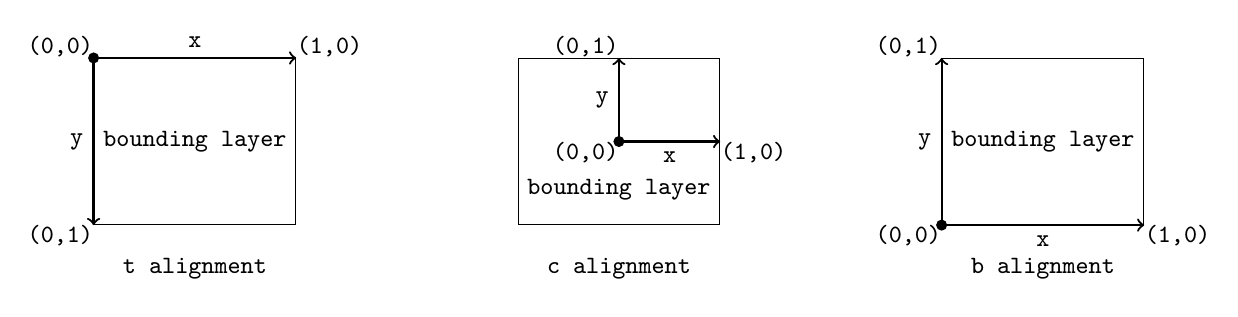
\begin{tikzpicture}[box/.style={draw, minimum width=6em, minimum height=6em},font={\tt\small}]
    \node[box] (t) {bounding layer};
    \node[below=2ex] at (t.south) {\texttt{t} alignment};
    \begin{scope}[shift=(t.north west), x=(t.north east), y=(t.south west)]
      \fill (0,0) circle (2pt);
      \draw[thick,->] (0,0) -- (1,0) node [midway,above] {x};
      \draw[thick,->] (0,0) -- (0,1) node [midway,left] {y};
      \node at (0,0) [above left,inner sep=0pt] {(0,0)};
      \node at (0,1) [below left,inner sep=0pt] {(0,1)};
      \node at (1,0) [above right,inner sep=0pt] {(1,0)};
    \end{scope}

    \node[box, right=8em, text height=4em] at (t.east) (c) {bounding layer};
    \node[below=2ex] at (c.south) {\texttt{c} alignment};
    \begin{scope}[shift=(c), x=(c.east), y=(c.north)]
      \fill (0,0) circle (2pt);
      \draw[thick,->] (0,0) -- (1,0) node [midway,below] {x};
      \draw[thick,->] (0,0) -- (0,1) node [midway,left] {y};
      \node at (0,0) [below left,inner sep=0pt] {(0,0)};
      \node at (0,1) [above left, inner sep=0pt] {(0,1)};
      \node at (1,0) [below right,inner sep=0pt] {(1,0)};
    \end{scope}


    \node[box, right=8em] at (c.east) (b) {bounding layer};
    \node[below=2ex] at (b.south) {\texttt{b} alignment};
    \begin{scope}[shift=(b.south west), x=(b.south east), y=(b.north west)]
      \fill (0,0) circle (2pt);
      \draw[thick,->] (0,0) -- (1,0) node [midway,below] {x};
      \draw[thick,->] (0,0) -- (0,1) node [midway,left] {y};
      \node at (0,0) [below left,inner sep=0pt] {(0,0)};
      \node at (0,1) [above left,inner sep=0pt] {(0,1)};
      \node at (1,0) [below right,inner sep=0pt] {(1,0)};
    \end{scope}
  \end{tikzpicture}
  \end{center}

  
\end{envwithcontents}
\begin{environment}{{layers<>}
    \oarg{parameter spec}\marg{code}\opt{\texttt{[<}\meta{default specification}\texttt{>]}}}
  This is a synonym for |\begin{incrementallayers} ... \end{incrementallayers}|.
\end{environment}





\section{Incremental alignment environments}\label{sec:align}

Standard \LaTeX\ alignment environments including |tabular| and the \texttt{align}
and \texttt{align*} environments from the \texttt{amsmath} package are not
ordinarily increment-aware.  The current package introduces a partial fix for
this, although their are remaining fragilities that may need to be worked
around.  It is possible to make an increment-aware version of any alignment
environment using |\CreateIncrementalAlignmentEnvironment| as described below.
However, a few such environments are defined automatically when |beamincr| is
loaded and these are described first, thus illustrating the behaviour once an
increment-aware environment has been created.

\vskip 2ex
\noindent
The following four environments are equivalent, apart from equation numbering:
\begin{environment}{{incrementalalign}\opt{\texttt{[<}\meta{spec1}\texttt{>\&<}\meta{spec2}\texttt{>\& ...]}}}
\end{environment}
\begin{environment}{{align<>}\opt{\texttt{[<}\meta{spec1}\texttt{>\&<}\meta{spec2}\texttt{>\& ...]}}}
\end{environment}
\begin{environment}{{incrementalalign*}\opt{\texttt{[<}\meta{spec1}\texttt{>\&<}\meta{spec2}\texttt{>\& ...]}}}
\end{environment}
\begin{environment}{{align*<>}\opt{\texttt{[<}\meta{spec1}\texttt{>\&<}\meta{spec2}\texttt{>\& ...]}}}
  Each pre-processes the input to |align[*]| to place an |\action<>{}| command
  around each field, defined as the material appearing between successive |&|
  and/or |\\| tokens.  By default, the first field on a line is called with
  |\action<+->{}|, and up to 7 remaining ones with |\action<.->{}|.  This has
  the effect of displaying a full line at a time, unless it has more than 8
  fields.  The optional argument makes it possible to change this behaviour to
  |\action<|\opt{\meta{spec1}}|>|, |\action<|\opt{\meta{spec2}}|>|, etc.\ with
  the sequence of specifications reset to |<|\opt{\meta{spec1}}|>| at the
  beginning of every line. If there are fewer specifications in the default than
  fields on a single line, these sequence is repeated.  The default
  specification values can be changed by calling
  |\setincrementalenvspec{align*}{<new defaults>}| or similar.

  The default specification for a single field can be overridden by placing a
  field-specific specification in |<>| at its start.  This means that a
  leading |<| in the field contents itself must be protected, e.g.\ by preceding
  it with |{}|.

  The use of |\action| means that beamer will interpret both standard
  |action@|\meta{increment} actions and implicit ones such as |!|-prefixed
  increment resets or |=| label assignments.
  \example
\begin{verbatim}
  \begin{align*<>}[<+->&<.->] % increment after every two &s
    x\incrlabel{x} &= y  &  1 &{}< 2 \\
    </x/-> x^2 &= y^2    &  <!/x/-> e^{i\pi} &<+->= -1 \\
    \sum_n f(n) &<.-|alert@.> \to \int f(x) dx
  \end{align*<>}
\end{verbatim}
    
    The pre-processor is not able to distinguish between the |&| alignment
    characters that apply to the containing environment and any that appear
    within enclosed environments, such as |array|.  Thus, any such environments
    must be protected using either a token register or a protected macro.  It is
    still possible to use increments within the environments: these are
    processed sequentially with those in the containing |align| environment,
    respecting increment labels, resets etc.

    \example
\begin{verbatim}
  % using token registers
  \newtoks\mymatrix
  \mymatrix={\begin{pmatrix} 1 & 2 \\ \alt<+->{3}{2} & 4 \\ \end{pmatrix}}
  \begin{align<>}
    \incrlabel{mat}\the\mymatrix \resetincr[/mat/]& \text{is \only<+->{not }singular}
  \end{align<>}

  % using \protected
  \protected\def\mymatrix{\begin{pmatrix} 1 & 2 \\ \alt<+->{3}{2} & 4 \\ \end{pmatrix}}
  \begin{align<>}
    \incrlabel{mat}\mymatrix \resetincr[/mat/]& \text{is \only<+->{not }singular}
  \end{align<>}

\end{verbatim}
    It may be wise to put the |\newtoks| declaration outside the frame so as not
    to consume more of \TeX's resources than needed.  

    |\intertext| lines must be terminated with |\\|.  By default they will be
    grouped within the action call of the last field of the preceding line.
    This behaviour can be changed by inserting a |\\| between that field and the
    |\intertext|.  By default, both |\\|s will add extra vertical space and an
    equation number in non-starred environments.  These can be avoided by using
    a form like |\nonumber\\[-3ex]| instead.

    At present, equation numbers aren't overlay aware.
\end{environment}
%
The incremental forms |incrementalgather|, |gather<>|, |incrementalgather*| and
|gather*<>| are also created when |beamincr| is loaded.  Although these contain
only one field per line, automatic access to \beamer\ and |beamincr| actions as
these lines are processed can be useful.  By default, they uncover equations a
line at a time (using |<+->|).

\begin{environment}{{incrementaltabular}\oarg{pos}\marg{cols}\opt{\texttt{[<}\meta{spec1}\texttt{>\&<}\meta{spec2}\texttt{>\& ...]}}}
\end{environment}
\begin{environment}{{tabular<>}\oarg{pos}\marg{cols}\opt{\texttt{[<}\meta{spec1}\texttt{>\&<}\meta{spec2}\texttt{>\& ...]}}}
  These provide increment-aware versions of the standard \LaTeX\ |tabular|
  environment.  By default, the entire table is uncovered on the current
  increment (using |<.->|), but this behaviour can be altered by changing the
  default specification when called, or by using |\setincrementalenvspec| as
  described below.  It may also be desirable to uncover entries
  column-by-column.  This effect can be achieved using increment labels.
  \example
\begin{verbatim}
\begin{tabular<>}{cccc}[</col1-/>&</col2-/>&</col3-/>&</col4-/>]
  <=(1)>/col1/\bf fruit & <=(2)>/col2/\bf colour  
      & <=(3)>/col3/\bf climate & <=(4)>/col4/\bf family \\[1ex]
  Apple & green & cool & pome \\
  Peach & yellow & warm & drupe \\
  Plum & purple & cool & drupe \\
  Orange & orange & hot & citrus \\
\end{tabular<>}  
\end{verbatim}
\end{environment}

\begin{environment}{{incrementaltabular*}\oarg{pos}\marg{width}\marg{cols}\opt{\texttt{[<}\meta{spec1}\texttt{>\&<}\meta{spec2}\texttt{>\& ...]}}}
\end{environment}
\begin{environment}{{tabular*<>}\oarg{pos}\marg{width}\marg{cols}\opt{\texttt{[<}\meta{spec1}\texttt{>\&<}\meta{spec2}\texttt{>\& ...]}}}
  These forms add the \meta{width} argument of \LaTeX's |tabular*| environment.
\end{environment}


\begin{command}{{\CreateIncrementalAlignmentEnvironment}\marg{base}\oarg{Nopts}\marg{Nreqs}\opt{\texttt{[<}default
      specification\texttt{>]}}}
  Create an increment-aware version of an alignment environment.  The \meta{base}
  environment should process its contents in fields demarcated by |&| and/or
  |\\| tokens.  The arguments \meta{Nopts} and \meta{Nreqs} specify the
  numbers of optional and required arguments the base environment expects.  If
  \meta{Nopts} is omitted it is taken to be 0.  \meta{Nreqs} must be
  specified, but can be 0.  If the \meta{default specification} is omitted it is
  set to |<.->|, thus displaying the environment contents at the prevailing
  increment number in the frame.

  The new environment can be accessed using either of the names
  |incremental|\meta{base} or \meta{base}|<>|.
\end{command}


\begin{command}{{\useincrementalenv}\marg{name}}
  Make all subsequent uses of the |name| environment call the incremental
  version.  The incremental version must already have been created.
  \example
\begin{verbatim}
\useincrementalenv{align*}
\begin{align*}[<+->]
  % this is an incremental environment
\end{align*}
\end{verbatim}
\end{command}

\begin{command}{{\usenonincrementalenv}\marg{name}}
  Restore the normal non-incremental behaviour of  subsequent |name| environments.
\end{command}


\begin{command}{{\setincrementalenvspec}\marg{name}\marg{default specification}}
  Set the default specification for incremental environments of type |name|.
\end{command}



\section{Pointing at things}\label{sec:point}

\begin{command}{\point\sarg{overlay specification}\marg{contents}}
  In normal text, insert a pointer before \meta{contents} on the specified
  slides.  If \meta{contents} includes any |\point*| commands, pointers are
  inserted at the locations of these commands at the same time.

  If called within a \TikZ\ picture, the |\point| command does not insert a
  pointer itself.  Instead, any pointer defined by the \texttt{pointer} option
  to any nodes in \meta{contents} is activated.  See the description of
  \texttt{pointer} below.
\end{command}

\begin{command}{{<point@}\opt{spec}\textcolor{red}{\tt >}}
  The action form of |\point| can be used in all contexts where an action
  specification is valid.  Its behaviour around normal text or \TikZ\ code is as
  above.  In \texttt{itemize} environments it replaces the default item label
  with the pointer\footnote{Although if the \texttt{itemize} is nested within an
    \texttt{enumerate}, it inherits the \texttt{enumerate} behaviour.}.  In
  \texttt{enumerate} environments it prepends the pointer to the default label.
  In other list environments, or when the label is set explicitly as an optional
  argument to |\item|, it has no direct effect.  However any |\point*| commands
  in the item label or text are activated.
\end{command}

\begin{command}{\point*}
  Insert a pointer when an enclosing |\point| command or action is active.
\end{command}

\begin{command}{{pointer}\opt{=}\oarg{pointer node options}\opt{\meta{angle}}}
  This is a \TikZ\ option that can be passed to a \texttt{node} to insert a
  pointer drawn towards the node whenever an enclosing |\point| command or
  action is active.  If an \meta{angle} is specified, the pointer is drawn
  towards the corresponding point on the node boundary; this can be specified as
  a numerical angle or a direction like \texttt{north}.  The default angle is
  \texttt{west} or \texttt{180}, so that the pointer points to the node from the
  left.  The pointer itself is drawn within a node: this behaviour is very
  similar to the regular \TikZ\ node \texttt{label} option, except that the
  pointer node is automatically sloped so as to point inwards.

  The current implementation does not work well with \texttt{coordinate}s.  The
  alternative \texttt{pointer coordinate} style creates an empty circular node
  of 0.1pt size, which is broadly equivalent.

  If \meta{pointer node options} are specified (generally requiring braces
  around the entire option value to protect \TikZ's option parsing from seeing
  the |[]|s) these are passed to the pointer node.  A few options may be
  particularly useful:
  \begin{description}
    \item[\tt pos=\meta{scale}] adjusts the placement of the pointer as a
      fraction of the distance from the target node centre to its boundary.  The
      default is 1.0.  This option is unlikely to be useful when the target is a
      \texttt{pointer coordinate}.
    \item[\tt pointer sep=\meta{dimen}] adds \meta{dimen} to the distance of the
      pointer from the target node.
    \item[\tt rotate=\meta{angle}] rotates the pointer relative to its initial
      angle.
  \end{description}

\end{command}


\begin{command}{\pointtonode\oarg{{\tt pointer} options}\marg{contents}}
  This is shorthand for
\begin{verbatim}
  \tikz[baseline]\node[anchor=base,text height=1.5ex,inner sep=0pt,pointer={#1}]{#2};
\end{verbatim}
The spacing adjustments ensure that the contents in the node are printed in
alignment with the surrounding text, and that pointers to an empty node appear
at a similar height to those inserted by |\point| or |\point*|.  The
availability of \meta{{\tt pointer} options} provides flexibility in the pointer
placement.
\end{command}

\begin{command}{\usepointer\oarg{inactive glyph}\marg{pointer glyph}}
  Use \meta{pointer glyph} for subsequent pointers in the current group.  If the
  optional argument is absent, then the pointer is replaced by a phantom of the
  same size when inactive (the size only matters if |\useuncoverpointer| is
  active).  If it is given, then inactive pointers are replaced by
  \meta{inactive glyph} (which may be empty).  \example
\begin{verbatim}
\usepointer{\raisebox{0.3ex}{\alert{$\blacktriangleright$}}} % the default
\usepointer{\raisebox{-0.4ex}{\alert{\HandRight}}} % requires \usepackage{bbding}
\end{verbatim}
Note that some adjustment of the vertical placement, as in these examples, may
be necessary to align the pointer appropriately with the text.

The effect of this command is local to the containing group. 

The pointer appearance should really be controlled through \beamer's template
mechanism, but that's a project for another day.
\end{command}

\begin{command}{\useoverprintpointer}
  Print subsequent pointers (and any inactive glyphs) in the current group
  \emph{over} existing material, without reserving any space for them
  (internally, they set within a zero-width box). This is the default, and
  avoids the dilemma of either leaving blank spaces for inactive pointers, or
  having text rearrange when the pointer appears.

  The effect of this command is local to the containing group. 
\end{command}

\begin{command}{\useuncoverpointer}
  Set subsequent pointers and any inactive glyph in the current group as normal
  text, taking up space on the page.  If no inactive glyph has been specified,
  the effect is to leave a blank space when the pointer is inactive, much like
  the effect of the |\uncover| or |\onslide| commands.  If the inactive glyph is
  set to the empty string, there is no blank space, but surrounding text is
  rearranged to make room for the pointer when it becomes active.

  The effect of this command is local to the containing group. 
\end{command}

\section{Misc helper functions}\label{sec:helper}

These functions may prove useful under some circumstances.

\begin{command}{\handoutframe\oarg{mode spec}\sarg{overlay specification}\marg{frame label}}
  This command only produces output when compiled in \meta{mode spec} (which
  defaults to \texttt{handout}, but can include more than one, e.g.,
  \texttt{[beamer$\mid$handout]}), in which case it renders the specified
  overlays from the named frame.  If \meta{overlay specification} is omitted,
  all the overlays are rendered.  The code works by switching temporarily to
  \texttt{beamer} mode as that seems to be the only way to produce more than one
  overlay per frame in \texttt{handout}, \texttt{trans} and \texttt{article}
  modes, although this means it may behave poorly with any mode-specific
  material within the frame.  The idea is from
  \url{https://tex.stackexchange.com/questions/455444/beamer-overlays-and-handout-exclude-frames-from-handout/455459#455459}.
\end{command}

Unfortunately,  the natural code
\example
\begin{verbatim}
\begin{frame}<handout:0>[label=twolists]
  ...
\end{frame}
\handoutframe<1,/halfway/,/done/>{twolists}
\end{verbatim}
fails, because the |<handout:0>| spec stops the increment labels from being
defined.  If running a recent \LaTeX\ compiler (post 2021) the command
|\framescanonly<handout>| described below provides a workaround.
\example
\begin{verbatim}
\begin{frame}[label=twolists]
  \framescanonly<handout|trans>%
  ...
\end{frame}
\handoutframe[handout|trans]<1,/halfway/,/done/>{twolists}
\end{verbatim}


\begin{command}{\framescanonly\opt{\sarg{mode specification}}}
  Scan the current frame without producing any output.  This is similar to a
  |<mode:0>| specification to |\begin{frame}|, but as the frame is still scanned
  it allows side effects such as increment label definitions.  The |\framescanonly|
  command should be placed inside the frame contents.  It is only available in
  recent versions of \LaTeX\ with hook support; a warning is printed in other
  cases.  If used in |beamer| mode the frame will be reprocessed for every
  overlay.  This behaviour can be avoided by also including a |<beamer:1>| or
  |<beamer:-1>| (but not |<beamer:0>|!) or equivalent specification to
  |\begin{frame}|. although it may be useful to fully expand advanced increment
  references when increments are reset (see \cref{sec:actions:advanced}).

  An example use appears above.
\end{command}

\begin{command}{\allowframescanonly\oarg{flag}}
  This commands disables (with \meta{flag} = 0) or enables (with \meta{flag} >
  0 or omitted) the effect of |\framescanonly|.  
\end{command}


\begin{command}{\beamincrdebug \marg{flag}}
  Turn on (\meta{flag} > 0) or off (\meta{flag} = 0) debugging mode.  When on,
  compilation generates messages in the terminal output and log file describing
  the rewriting actions that |beamincr| performs.
\end{command}




\section{Internals}\label{sec:internals}

These sections discuss more background and some implementation details.   This
is only likely to be of interest to users who wish to extend the approach.

\subsection{Pauses, increments and the \texttt{beamerpauses} counter}

Both |\pause| and incremental overlay specifications access the same underlying
counter called |beamerpauses|, but they use them in different ways.

\begin{command}{\pause}
  increments |beamerpauses| and then sets subsequent material on the slide
  given by the incremented |\value{beamerpauses}|. 
\end{command}

\begin{command}{\onslide\texttt{<+->}}
  increments |beamerpauses| but then sets subsequent (or argument) material on
  the slide corresponding to the \emph{previous} value of |beamerpauses|.
\end{command}

\begin{command}{\onslide\texttt{<.->}}
  leaves |beamerpauses| alone, but sets subsequent (or argument) material on the
  slide given by |\value{beamerpauses}-1|, unless |\value{beamerpauses}=1| in
  which case it puts subsequent material on slide 1.
\end{command}
%
This conflict in interpretation of the |beamerpauses| counter can cause
unintuitive effects.  The incremental specfication model is far more flexible
and powerful, and so the commands of this package can all be interpreted in
terms of an \emph{increment number} which ordinarily equals
|max(\value{beamerpauses}-1,1)|.  In fact, internally they all use the
|beamerpauses| counter with this offset.  Thus, when commands like |\resetincr|
set the increment value, they set |beamerpauses| to the increment + 1.  This
value then behaves sensibly with |<+>| etc.\ specifications, but not with
|\pause|.

An exception is when the current increment is set to 0, either explicitly or by
using an advanced (or otherwise undefined) increment reference.  In this case
|beamerpauses| is also set to 0, not 1.  This is because |beamincr| references
use the 0 value to detect the undefined reference, and so suppress offsets and
ranges as described in \cref{sec:actions:advanced}.  However, subsequent uses of
\beamer's |<+>| specification will increment |beamerpauses|, potentially placing
text on earlier slides than intended.  This behaviour can be avoided (at the
expense of more typing) by using |<!/.(1)/>| instead.


\subsection{Overlay specification parsing routines}

The |beamincr| overlay specification extensions work by injecting various
parsing routines into the core \beamer\ parser (called |\beamer@masterdecode|),
before calling the original function.  These parsers are also available as user
commands, and may be helpful for debugging (though see also |\beamincrdebug|
above).  

\begin{command}{\parsedefincspec \marg{overlay spec}}
  Replace any \texttt{|\~{}|} fields in \meta{overlay spec} with the current
  default specification.
\end{command}
  
\begin{command}{\parseincrspec \marg{overlay spec}}
  Interpret any text enclosed in |/|s within \meta{overlay spec} as an increment
  specification, replacing each with the corresponding numerical values
  (including offset).  Also processes any open ranges internal to the label as
  described in \cref{sec:actions:advanced}.
\end{command}

\begin{command}{\parseresetspec \marg{overlay spec}}
\end{command}

\begin{command}{\parselabelspec \marg{overlay spec}}
\end{command}




% for reference with \slideref{foo} (and/or </foo/>).
%
% The "increment number" is defined by the use of \pause and relative
% overlay commands like \onslide<+->.  In general, it corresponds to the slide
% on which text that followed the most recent <+> increment would
% appear.  For technical reasons this is one less than the value of the
% beamerpauses counter (unless that counter is 1).  This can cause confusion if
% \pause and <+> constructs are mixed.  

% the internal label name includes the frame label if one is given -- this helps
% to keep the references valid across frames



% \bibliographystyle{apalike} 
% \bibliography{journalsabbrv,neuro,learning}

\end{document}

% Local Variables:
% mode: latex
% eval: (set-fill-column 80)
% End:
